\section{Experimental Results}\label{sec:4}%
\newcommand{\car}[1]{\emph{#1}}%

The drivers were developed in C++\footnote{Code available at \url{https://github.com/bruno147/fsmdriver}} and tested in TORCS\footnote{\url{http://sourceforge.net/projects/torcs/}} (v1.3.6) and SCR\footnote{\url{http://sourceforge.net/projects/cig/files/SCR\%20Championship/Server\%20Linux/}} (v2.1). The car used in the experiments was \car{car1-trb1}, the standard model for SCR~\cite{SCR}.

\gnramos{que formula eh essa? nao esta na referencia (pelo menos nao deste jeito. a ideia eh saber exatamente a referencia/pagina/linha que originou este valor  de 616}
% G = 267,43*ln(P) - 293,21 (G = generations, N = population size)
The FSMDrivers' parameters are evolved through a genetic algorithm, aiming to improve their racing performances by changing their values. The GA used standard configurations from literature, the population size was arbitrarily set as 30~\cite{RATES}, which leads to 616 generations for a moderate problem complexity in which the optimal population size was coded as bitstrings~\cite{218485}. Selection is done through elitism by keeping the best 4 individuals from a generation unchanged, and the other 26 are generated from the best 10 individuals' reproduction. This step is done by randomly choosing a pair from the top 10 that are cloned with a 5\% chance or generate a pair of offspring with a 95\% probability~\cite{RATES}. These offspring are produced through crossover by partitioning the parents' bitstrings at a random position and swapping them. Finally, mutation (a simple bit flip) is applied to every bit in every individual of these 26 with a 1\% probability~\cite{RATES}.

The fitness of each individual is computed as the distance covered in the race. The GA communicates with the test platform, simulating races with the drivers in the desired tracks in TORCS, through operating system calls to the command line interface and the fitness communicated through shared memory\footnote{Code available at \url{https://github.com/bruno147/driver-ga}}.

The two FSMDriver models had their parameters evolved through the GA and compared to each other. This considers only the \racing~states, as \OT~and \St~are considered adequate with the manual settings. During this evolution, the learning module in FSMDriver3 is disabled in order to not interfere with the learning, and no parameter in the module was included model's bitstring representation. To analyze the learning module's effect, two instances of the 3-state FSM controller were tested, the FSMDriver3+ with it enabled, and disabled in FSMDriver3. When enabled, the learning module's threshold speed is arbitrarily set to 85 km/h. All controllers have 5 laps for warm-up, during which they can adapt to the track, in accordance to the stipulated 2015 Championship rules\footnote{\url{http://cs.adelaide.edu.au/~optlog/SCR2015/}}.

\newcommand{\profile}[1]{\emph{#1 driver}}%
Since it is unknown which tracks will be used during the SCR Championship, a more general and versatile controller is desirable and, thus, the controllers were evolved considering their performance in several tracks types. Three basic driver profiles were desired: a \profile{road}, which should perform well in \track{road} and \track{oval} tracks, a \profile{dirt}~for \track{dirt} roads and a \profile{mixed}, which should perform well in both types.

For the \profile{road} profile, four road tracks were selected from the standard TORCS distribution list to compose the training set in the evolution process. The tracks were arbitrarily selected for certain features, which might lead to better drivers: \track{Spring}, the longest track available; \track{Wheel 2}, with many sharp curves; \track{E-Track 3}, a fast track with sharp curves; and \track{Forza}, a fast circuit with smoother curves.

Analogously, four dirt tracks were selected for evolving a \profile{dirt profile}: \track{Dirt 2}, \track{Dirt 6}, \track{Mixed 1}, and \track{Mixed 2}, which present variations of high speed and curve styles. For the \profile{mixed}, two of each were selected: \track{Spring}, \track{Wheel 2}, \track{Dirt 2}, and \track{Mixed 1}.

\begin{figure*}[t]
\centering
\begin{subfigure}[b]{0.15\textwidth}
       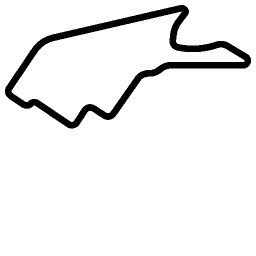
\includegraphics[width=\textwidth]{img/tracks/Street1}
       \caption{Street 1}
   \end{subfigure}
\begin{subfigure}[b]{0.15\textwidth}
       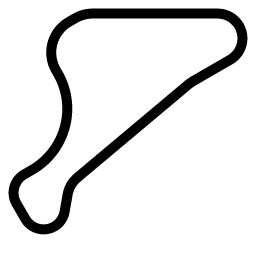
\includegraphics[width=\textwidth]{img/tracks/CG-Speedway}
       \caption{CG Speedway number 1}
   \end{subfigure}
\begin{subfigure}[b]{0.15\textwidth}
       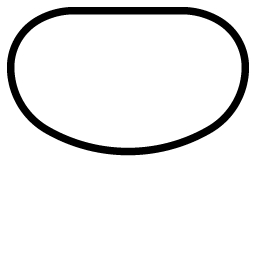
\includegraphics[width=\textwidth]{img/tracks/D-Speedway}
       \caption{D-Speedway}
   \end{subfigure}
\begin{subfigure}[b]{0.15\textwidth}
       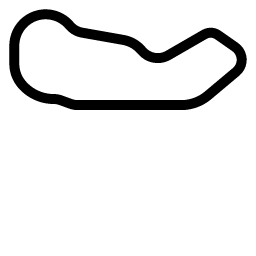
\includegraphics[width=\textwidth]{img/tracks/Dirt1}
       \caption{Dirt 1}
   \end{subfigure}
\begin{subfigure}[b]{0.15\textwidth}
       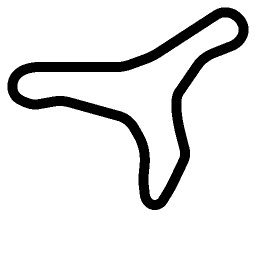
\includegraphics[width=\textwidth]{img/tracks/Dirt3}
       \caption{Dirt 3}
   \end{subfigure}
\begin{subfigure}[b]{0.15\textwidth}
       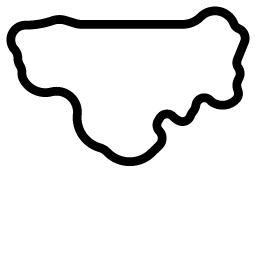
\includegraphics[width=\textwidth]{img/tracks/Dirt4}
       \caption{Dirt 4}
   \end{subfigure}
   \caption{Test tracks, road tracks (a, b), oval (c), and dirt tracks (d, e, and f)~\protect\cite{TORCS}.}\label{fig:tracks}
\end{figure*}

The best solutions evolved for each profile where then evaluated in a set of six tracks, different from the ones used before, which present distinct typed, speeds, and curve features for better analysis. These tracks, shown in Figure~\ref{fig:tracks} and available on the standard TORCS set, were used in previous SCR Championships~\cite{AUTOPIA2009}. They are two road tracks: \track{Street 1} and \track{CG Speedway 1}; one oval track: \track{D-Speedway}; and three dirt tracks: \track{Dirt 1}, \track{Dirt 3}, and \track{Dirt 4}.

%%%%%%%%%%%%%%%%%%%%%%%%%%%%%%%%%%%%%%%%%%%%%%%%%%%%%%%%%%%%%%%%%%%%%%%%%%%%%%%%
\subsection{Single Race Results}
\begin{table*}[!btp]
% \renewcommand{\arraystretch}{1.3}
\caption{Distance covered (in meters) racing alone for 10.000 game ticks.}\label{tbl:ticks}
\centering
\begin{tabular}{| c | c || c | c | c | c | c | c |}
\cline{3-8}
\multicolumn{2}{ c | }{} & \multicolumn{6}{ c |}{\bfseries Track} \\\hline
\multicolumn{2}{| c ||}{\bfseries Driver} & \bfseries\track{Street 1} & \bfseries\track{CG Speedway number 1} & \bfseries\track{D-speedway} & \bfseries\track{Dirt 1} & \bfseries\track{Dirt 3} & \bfseries\track{Dirt 4} \\\hline\hline
\multirow{3}{*}{FSMDriver5}
& road  & 3822.76 & 4114.66 & 3427.11 & 2145.49 & 2205.97 & 3260.19 \\\cline{2-8}
& dirt  & 1267.83 & 2057.47 & 2936.82 & 1072.92 & 2205.82 & 3260.33 \\\cline{2-8}
& mixed & 3822.99 & 4114.80 & 3427.06 & 2145.75 & 2205.83 & 3260.31 \\\hline\hline
\multirow{3}{*}{FSMDriver3}
& road  & \textbf{7925.60} & 8745.49 & 13196.50 & 3978.01 & 3451.26 & \textbf{6757.83} \\\cline{2-8}
& dirt  & 5103.41          & 5093.82 &  8589.13 & 3525.84 & 4905.58 & 5590.78 \\\cline{2-8}
& mixed & 5864.48          & 8714.58 & 11694.60 & 5052.38 & 4920.32 & 3797.83 \\\hline\hline
\multirow{3}{*}{FSMDriver3+}
& road  & 7532.93 & 8804.73 & 10720.20 & 3678.89          & 5199.46          & 3193.44 \\\cline{2-8}
& dirt  & 4738.76 & 5102.92 &  8197.55 & 3525.84          & 4214.30          & 5057.18 \\\cline{2-8}
& mixed & 6780.43 & 8089.41 & 10943.10 & \textbf{5752.90} & \textbf{5824.93} & 5614.62 \\\hline\hline
\multicolumn{2}{| c ||}{AUTOPIA~\cite{AUTOPIA2009}} & 7091.8 & \textbf{8970.4} & \textbf{15612.3} & * & * & * \\\hline
\end{tabular}
\end{table*}

Table~\ref{tbl:ticks} presents the distance covered results for these tests for each FSMDriver model and profile (best results per track in bold). The fitness function in this case is the sum of distances covered in all tracks, considering 10.000 game ticks per track, as per the SCR rules, so higher values are desirable. The table also includes, for direct comparison with the current state of the art, results for AUTOPIA in three of the same tracks for the same 10.000 game ticks metric, as presented in~\cite{AUTOPIA2009}. The `*' symbol indicates that the driver does not have data available for the track.

Considering the 5-states FSMDriver in \track{road}/\track{oval} tracks, it is clear that the \profile{road} and \profile{mixed} have better results than \profile{dirt}, since this profile uses road tracks for evaluating individuals during evolution. Looking at the results for \track{dirt} tracks, all profiles have similar performances except for the \profile{dirt} in \track{Dirt 1}. \gnramos{por que? relacionado ao formato da pista?} FSMDriver5's \profile{road} and \profile{mixed} are practically equivalent and at least as good as its \profile{dirt}, and all profiles are quite inferior to the other controllers shown in Table~\ref{tbl:ticks}.

Looking at FSMDriver3 in \track{road}/\track{oval} tracks, it is also clear that the \profile{road} and \profile{mixed} have better results than \profile{dirt}, as was expected. Considering the results for \track{dirt} tracks, \profile{mixed}'s performance was significantly better than the others in \track{Dirt 1} and \track{Dirt 3}, but \profile{road} produced the best result in \track{Dirt 4}. \gnramos{por que? relacionado ao formato da pista?} \profile{road}'s result for \track{Street 1} was also the best all around.

FSMDriver3+ profiles (with learning module enabled) also performed as expected in \track{road}/\track{oval} tracks. For these, FSMDriver3+ had shorter distances than FSMDriver3 for \track{Street 1} (5\%) and \track{D-speedway} (18.8\%), and a slightly longer for \track{CG Speedway number 1} (0.7\%). This is also expected as the driver learns to slow down in order to stay in the track. For \track{dirt} tracks, FSMDriver3+'s \profile{mixed} had the best results, better than FSMDriver3 for \track{Dirt 1} (13.9\%) and \track{Dirt 3} (18.4\%), though worse in \track{Dirt 4} (16.9\%). \gnramos{os resultados para Dirt 4 estao certos?}

Comparing the results for \track{road}/\track{oval} tracks with AUTOPIA (\cite{AUTOPIA2009}), the current state of the art in SCR, FSMDriver3's \profile{road} was about 11.8\% better in \track{Street 1} while FSMDriver3+ was 6.2\% better. In \track{CG Speedway number 1}, FSMDriver3 and FSMDriver3+ were only 2.5\% and 1.8\% worse, respectively. In \track{D-speedway}, these numbers rise to 15.5\% and 31.3\%. Thus, the 3-state FSMDriver model showed potential for competing on \track{road} tracks.

In order to learn more about FSMDriver's endurance, a new set of tests using the distance raced in 10 laps as metric was executed, and the results presented in Table~\ref{tbl:time}. The values represent the time needed to complete the laps, so lower values are desirable, the `\textdagger'~symbol indicates that the driver does not complete the 10 laps required, and the `*' symbol indicates that the driver does not have data available for the track.

\begin{table*}[!btp]
	% \renewcommand{\arraystretch}{1.3}
\caption{Time elapsed (in seconds) racing alone for 10 laps.}\label{tbl:time}
\centering
\begin{tabular}{| c | c || c | c | c | c | c | c |}
	\cline{3-8}
\multicolumn{2}{ c | }{} & \multicolumn{6}{ c |}{\bfseries Track} \\\hline
\multicolumn{2}{| c ||}{\bfseries Driver} & \bfseries\track{Street 1} & \bfseries\track{CG Speedway number 1} & \bfseries\track{D-speedway} & \bfseries\track{Dirt 1} & \bfseries\track{Dirt 3} & \bfseries\track{Dirt 4} \\\hline\hline
\multirow{3}{*}{FSMDriver5}
& road  & \textdagger & 816.6       & \textdagger & \textdagger & \textdagger & \textdagger \\\cline{2-8}
& dirt  & \textdagger & \textdagger & \textdagger & \textdagger & \textdagger & \textdagger \\\cline{2-8}
& mixed & \textdagger & \textdagger & \textdagger & \textdagger & \textdagger & \textdagger \\\hline\hline
\multirow{3}{*}{FSMDriver3}
& road  & \textbf{1086.28} & \textbf{483.17} & \textbf{607.35} & \textdagger & 1150.09 & \textdagger \\\cline{2-8}
& dirt  & \textdagger      & 1274.81         & 840.02          & 597.33      & 1045.62 & 1307.52  \\\cline{2-8}
& mixed & 1096.95          & 510.86          & 612.00          & 408.57      & 811.96  & 2157.95 \\\hline\hline
\multirow{3}{*}{FSMDriver3+}
& road  & 1225.24 & 484.58  & 709.74 & \textdagger & 1108.48 & \textdagger \\\cline{2-8}
& dirt  & 1658.47 & 1291.31 & 915.86 & 597.33      & 1055.21 & 1360.71 \\\cline{2-8}
& mixed & 1208.84 & 534.87  & 646.68 & 384.93      & 939.93  & 1930.19 \\\hline\hline
\multicolumn{2}{| c ||}{Berniw Hist4} & 1143.77 & 605.76 & 656.24 & 460.95 & 872.97 & 1127.45 \\\hline\hline
\multicolumn{2}{| c ||}{AUTOPIA~\cite{AUTOPIA}}  & * & * & * & \textbf{339.3} & \textbf{742.4} & \textbf{796.5} \\\hline
\end{tabular}
\end{table*}

Table~\ref{tbl:time} also includes results for the robot \emph{Berniw Hist4}, provided in with the TORCS distribution. This was not included in the previous tests because TORCS only allows a race with the available robots to run for a given amount of laps (not game ticks). This robot has intermediate performance, and was arbitrarily chosen from other robots to provide insights on the controllers performance compared to a robot's and to AUTOPIA, as presented in ~\cite{AUTOPIA}. Direct comparison is not exactly fair because \emph{Berniw Hist4} does not the standard car \car{car1-trb1}, it uses the legacy \car{TZ2}.

Looking at results for FSMDriver5, only the \profile{road} completed 10 laps in \track{CG Speedway number 1}, all other instances had excessive damage. The 3-state FSMDriver, on the other hand, completed all track in at least 2 profiles.

Considering FSMDriver3 in \track{road}/\track{oval} tracks, it is also clear that the \profile{road} and \profile{mixed} have better results than \profile{dirt}, as expected. Considering the results for \track{dirt} tracks, \profile{mixed}'s performance was significantly better than the others in \track{Dirt 1} and \track{Dirt 3}, while \profile{dirt} was almost twice as fast in \track{Dirt 4}. \gnramos{por que? relacionado ao formato da pista?}

FSMDriver3+ profiles also performed as expected in \track{road}/\track{oval} tracks. For these, FSMDriver3+ required a longer time than FSMDriver3 for \track{Street 1} (12.8\%) and \track{D-speedway} (0.3\%), but it did finish \track{CG Speedway number 1} while FSMDriver3 did not. This is also expected as the driver learns to avoid leaving the track and, thus, receive damage. For \track{dirt} tracks, FSMDriver3+'s \profile{mixed} had better than FSMDriver3 for \track{Dirt 1} (5.8\%), but worse in \track{Dirt 3} (15.8\%) and \track{Dirt 4} (14.1\%).

Considering the robot \emph{Berniw Hist4}, it seems that the 3-state FSMDriver is better controller, despite the ``handicap'' of using SCR's interface for driving and not having access to additional information from the simulator (such as track layout).

Finally, comparing the results for \track{dirt} tracks with AUTOPIA (\cite{AUTOPIA}), FSMDriver3's \profile{mixed} was about 20.4\% worse in \track{Dirt 1} while FSMDriver3+ was 13.2\%. In \track{Dirt 3}, FSMDriver3 and FSMDriver3+ were only 9.4\% and 26.6\% worse, respectively. In \track{Dirt 4}, these numbers rise to 170.9\% and 142.3\%.

%%%%%%%%%%%%%%%%%%%%%%%%%%%%%%%%%%%%%%%%%%%%%%%%%%%%%%%%%%%%%%%%%%%%%%%%%%%%%%%%
\subsection{Analysis}
As expected, the controllers evolved on \track{road}/\track{oval} tracks were fastest. \track{dirt} tracks provide a more difficult environment, sudden braking often results in unwanted behavior, skidding is noticeably more common then. The controllers evolved in this end of the evolution process tends to drive in lower speeds to stay within track boundaries. \profile{Mixed}s tend to evolve some of the faster, reckless behavior for \profile{road}, while keeping some of the carefulness of a \profile{dirt}, producing intermediate results.

Though the FSMDriver5 configuration proposed seems intuitively correct, the performance - obviously - dependent which states are activated during the race, and, thus, how these states were handled in the evolution process. A more detailed analysis of race logs indicate that the parameters in the transition function, which define the current state, are very susceptible to the inputs, resulting in several changes in the states which greatly impacts the evolution of the states' parameters and, consequently, of those in the function. By having multiple states acting inside the track the 5-state model struggles to define the boundaries of different typed of track segments, and mismatching between perceived and actual states would often cause the car to leave the track.

This suggests a different approach to development, such as adjusting one state at a time (independently) and then the transition function or augmenting the FSM from a successful 3-state configuration. Additionally, the variance approach is also very sensitive to the car's position at the moment, implying that a different, more robust metric for establishing the type of track segment the car is in should be pursued. Another possibility, since the search space is larger than FSMDriver3's, is to increase the number of individuals and/or generations in the genetic algorithm's configurations.

Considering the 3-state model, it was seen that it quickly achieved an intermediate level performance in TORCS (compared to FSMDriver5 and \emph{Berniw Hist4}). The less complex finite state machine model is more compatible with the tested optimization method, since it has a 23\% smaller search space and with the simpler transition function, which enables completely independent evolution of the states.

Considering the 10.000 game ticks results, the learning module produces slightly slower drivers, but both FSMDriver3 and FSMDriver3+ had interesting results in all tracks tested, and they bested AUTOPIA's qualifying mark for \track{Street 1}. This is very significant because it implies that FSMDriver could qualify to the SCR Championship's racing stage (after the qualifying stage) ahead of the current state of the art.

Analyzing the results for 10 laps, FSMDriver5 has obviously poor driving skills for longer races, taking excessive damage and being unable to complete any. The 3-state models, on the other hand were able to finish the all tracks. FSMDriver3+ finished \track{Street 1} while FSMDriver3 did not, which could indicate that the learning module produces a more careful driver that takes less damage, prolonging its endurance (a desired feature during the race stage). \gnramos{eh preciso dados sobre os danos para poder argumentar alguma coisa aqui}. In these tests, AUTOPIA was clearly a better driver than the others, despite not having supremacy in the qualifying.

A visual comparison between FSMDriver and AUTOPIA in a simulation using TORCS graphical interface revealed that AUTOPIA's brake, acceleration and recovery policies are better than the ones achieved with FSMDriver. AUTOPIA barely leaves and track and is more stable in curves in \track{dirt} tracks.